% !TeX spellcheck = de_CH
\documentclass[
a4paper,
oneside,
10pt,
fleqn,
headsepline,
toc=listofnumbered, 
bibliography=totocnumbered]{scrartcl}

% deutsche Trennmuster etc.
\usepackage[T1]{fontenc}
\usepackage[utf8]{inputenc}
\usepackage[english, ngerman]{babel} % \selectlanguage{english} if  needed
\usepackage{lmodern} % use modern latin fonts

% Custom commands
\newcommand{\AUTHOR}{M. Wieland}
\newcommand{\SECONDAUTHOR}{F. Hauser}
\newcommand{\THIRDAUTHOR}{M. Trentini}
\newcommand{\FOURTHAUTHOR}{P. Scherler}
\newcommand{\INSTITUTE}{Hochschule für Technik Rapperswil}
\newcommand{\LECTURER}{Prof. Dr. Jürg Stadelwieser}
\newcommand{\GITHUB}{https://github.com/michiwieland/businessplan}

% Jede Überschrift 1 auf neuer Seite
\let\stdsection\section
\renewcommand\section{\clearpage\stdsection}

\makeatletter
\newcommand\invisiblesection[1]{%
	\refstepcounter{section}%
	\addcontentsline{toc}{section}{\protect\numberline{\thesection}#1}%
	\sectionmark{#1}\phantom{}}
\makeatother

% Multiple Authors
\usepackage{authblk}

% Include external pdf
\usepackage{pdfpages}

% Layout / Seitenränder
\usepackage{geometry}

% Inhaltsverzeichnis
\usepackage{makeidx} 
\makeindex

\usepackage{url}
\usepackage[pdfborder={0 0 0}]{hyperref}
\usepackage[all]{hypcap}
\usepackage{hyperxmp} % for license metadata

% Glossar und Abkürzungsverzeichnis
\usepackage[acronym,toc,nopostdot]{glossaries}
\glossarystyle{altlisthypergroup}
\usepackage{xparse}
\DeclareDocumentCommand{\newdualentry}{ O{} O{} m m m m } {
	\newglossaryentry{gls-#3}{name={#5},text={#5\glsadd{#3}},
		description={#6},#1
	}
	\makeglossaries
	\newacronym[see={[Siehe:]{gls-#3}},#2]{#3}{#4}{#5\glsadd{gls-#3}}
}
\makeglossaries

% Mathematik
\usepackage{amsmath}
\usepackage{amssymb}
\usepackage{amsfonts}
\usepackage{enumitem}

% Images
\usepackage{graphicx}
\graphicspath{{images/}} % default paths

%figures
\usepackage{tikz}
\usetikzlibrary{shapes.geometric}

%risk-rating
\newcommand\risk[2]{
	\begin{tikzpicture}
	\draw [thick, |->] (0,2) -- (#2,2);
	\draw [fill=red, thick] (#1,2) circle [radius=0.2];
	\end{tikzpicture}
}

% Boxes
\usepackage{fancybox}

%Tables
\usepackage{tabu}
\usepackage{booktabs} % toprule, midrule, bottomrule
\usepackage{array} % for matrix tables

% Multi Columns
\usepackage{multicol}

% Header and footer
\usepackage{scrlayer-scrpage}
\setkomafont{pagehead}{\normalfont}
\setkomafont{pagefoot}{\normalfont}
\automark*{section}
\clearpairofpagestyles
\ihead{\headmark}
\ohead{\TITLE}
\cfoot{\pagemark}

% Pseudocode
\usepackage{algorithm}
\usepackage{algorithmic}

% Code Listings
\usepackage{listings}
\usepackage{color}
\usepackage{beramono}

\definecolor{DarkPurple}{rgb}{0.4, 0.1, 0.4}
\definecolor{DarkCyan}{rgb}{0.0, 0.5, 0.4}
\definecolor{LightLime}{rgb}{0.3, 0.5, 0.4}
\definecolor{Blue}{rgb}{0.0, 0.0, 1.0}

\lstdefinestyle{eclipse-style}{
	language=Java,
	columns=flexible,
	showstringspaces=false,
	basicstyle=\footnotesize\ttfamily, 
	keywordstyle=\bfseries\color{DarkPurple},
	commentstyle=\color{LightLime},
	stringstyle=\color{Blue}, 
	escapeinside={£}{£}, % latex scope within code
	morekeywords={length},
	numbers=left,
	numberstyle=\tiny\color{black},
	frame=single,
}
\lstset{style=eclipse-style}


% Theorems \begin{mytheo}{title}{label}
\usepackage{tcolorbox}
\tcbuselibrary{theorems}
\newtcbtheorem[number within=section]{definiton}{Definition}%
{fonttitle=\bfseries}{def}
\newtcbtheorem[number within=section]{remember}{Merke}%
{fonttitle=\bfseries}{rem}
\newtcbtheorem[number within=section]{hint}{Hinweis}%
{fonttitle=\bfseries}{hnt}

% Dokumentinformationen
\newcommand{\SUBJECT}{Businessplan}
\newcommand{\TITLE}{GitFit}

% pdf metadata
\hypersetup{
	pdfauthor={\AUTHOR},
	pdftitle={\SUBJECT \TITLE}
}

\begin{document}


% German \and
\renewcommand\Authands{ und }
% Front page
\title{\TITLE}
\subject{\SUBJECT}
\author{\SECONDAUTHOR}
\author{\THIRDAUTHOR}
\author{\FOURTHAUTHOR}
\author{\AUTHOR}
\affil{\INSTITUTE}
\affil{\LECTURER}
\date{\today}
\maketitle

\pagecolor{PrimaryColor}\afterpage{\nopagecolor}

\begin{center}
	
\includegraphics[width=0.7\linewidth]{images/front}
\end{center}


\color{black}


% Table of contents
\tableofcontents


% Glossar and acronyms (if included \loadglsentries{glossar})
\printglossary[type=\acronymtype]
\printglossary
\glsaddall


%TODO Total: 20 Seiten
%TODO Gute Idee prüfen: Man verkauft keine Produkte/Dienstleistungen sondern Nutzen! 
%TODO -> Es muss ersichtlich sein, was das Produkt bringt.
%TODO Zugänglichkeit, Komfort, Image, Lifestyle, Trend

%TODO Buch: Business Model Generation

%TODO Sturktur nach PWC

% Kundenbedürfnisse
%K omfort
%A nsehen
%N euheiten
%S elbsterhaltig
%R isikolos
%O ekonomie (Geld, Zeit)
%O ekologie (Umweltverträglich, BIO)
%S ympathie (menschlich, Design)
%A ngehörigkeit, zugehörigkeit (Teil einer ausgewählten Gruppe)

% Check https://www.ige.ch/

% Feedback Präsentation:
% - Handys nicht gerne gesehen, Stellenabbau nicht interessant da oft wenige Mitarbeiter, 2 Big Player (Migros, Coop)

\section{Abstract}
% TODO Remove Example for bibliography entry
\cite{ackema:1998}


% TODO Wir bieten flexibiltät, effizienz, komfort


\section{Das Businessmodell}
%TODO Import Canvas \includepdf[pages={1},landscape=true]{appendix/schemes/datacenter.pdf}

\section{Mission, Vision und Strategie: die Zukunft}
\subsection{Mission}
Unsere Aufgabe ist es, vielen Menschen ein völlig neues Erlebnis für ein persönliches Training im Fitnesscenter zu bieten. Wir tun dies, indem wir eine App anbieten, welche die Fitnesslandschaft revolutioniert. Dies zu Preisen, die sich auch kleine Fitnesscenter leisten können.

\subsection{Vision}
Schweizer Fitnesscenter setzen aktuell vorzugsweise auf Papier und Bleistift für die Trainingsplanung ihrer Kunden. Dies ist nicht mehr zeitgemäss und bedarf einer Generalüberholung. Am Puls der Zeit zu sein, bedeutet für ein Fitnesscenter, einen modernen und attraktiven Dienstleister für seine Kunden darzustellen. Die Digitalisierung bietet unendlich viele Möglichkeiten, die es zu nutzen gilt. \\
Wir wollen eine App kreieren, welche die Fitnessbranche wieder auf den aktuellen Stand der Technik katapultiert. Die App bietet aufschlussreiche Statistiken sowie hilfreiche Tipps zur Übung, wenn der Trainer gerade nicht in der Nähe ist.

\subsection{Strategie}
Unser Angebot richtet sich in erster Linie an grosse Fitnesscenter-Ketten, da wir glauben, dass diese an einem übergreifenden Wissensaustausch der Filialen interessiert sind. Im Rahmen der Entwicklung kümmern wir uns in einer ersten Phase um das Anreichern von Stammdaten mit auserwählten Partner-Center. Die Daten sollen als solides und realitätsnahes Fundament für die weitere Entwicklung dienen. In einer zweiten Phase wird dann die App für den Endkunden entwickelt, die ein möglichst komfortables und persönliches Trainingserlebnis vermitteln soll. 

\subsubsection{Wettbewerbsstrategie}
Der Schweizer Fitnessmark boomt und trotzdem ist keine Digitalisierung in der Branche erkennbar. Ähnliche Projekte finden im Ausland bereits Anklang, jedoch gibt es im Inland keine vergleichbare Dienstleistung. Grund genug, diese Lücke zu füllen. Die Schwierigkeit in dem Projekt liegt deshalb weniger in der Positionierung gegenüber ausländischen Dienstleister, sondern vielmehr die heimischen Fitnesscenter mit der neuen Technologie vertraut zu machen.


\section{Produkte und Dienstleistungen: die Marktleistung}

\subsection{Die App}
\begin{figure}[h]
\centering
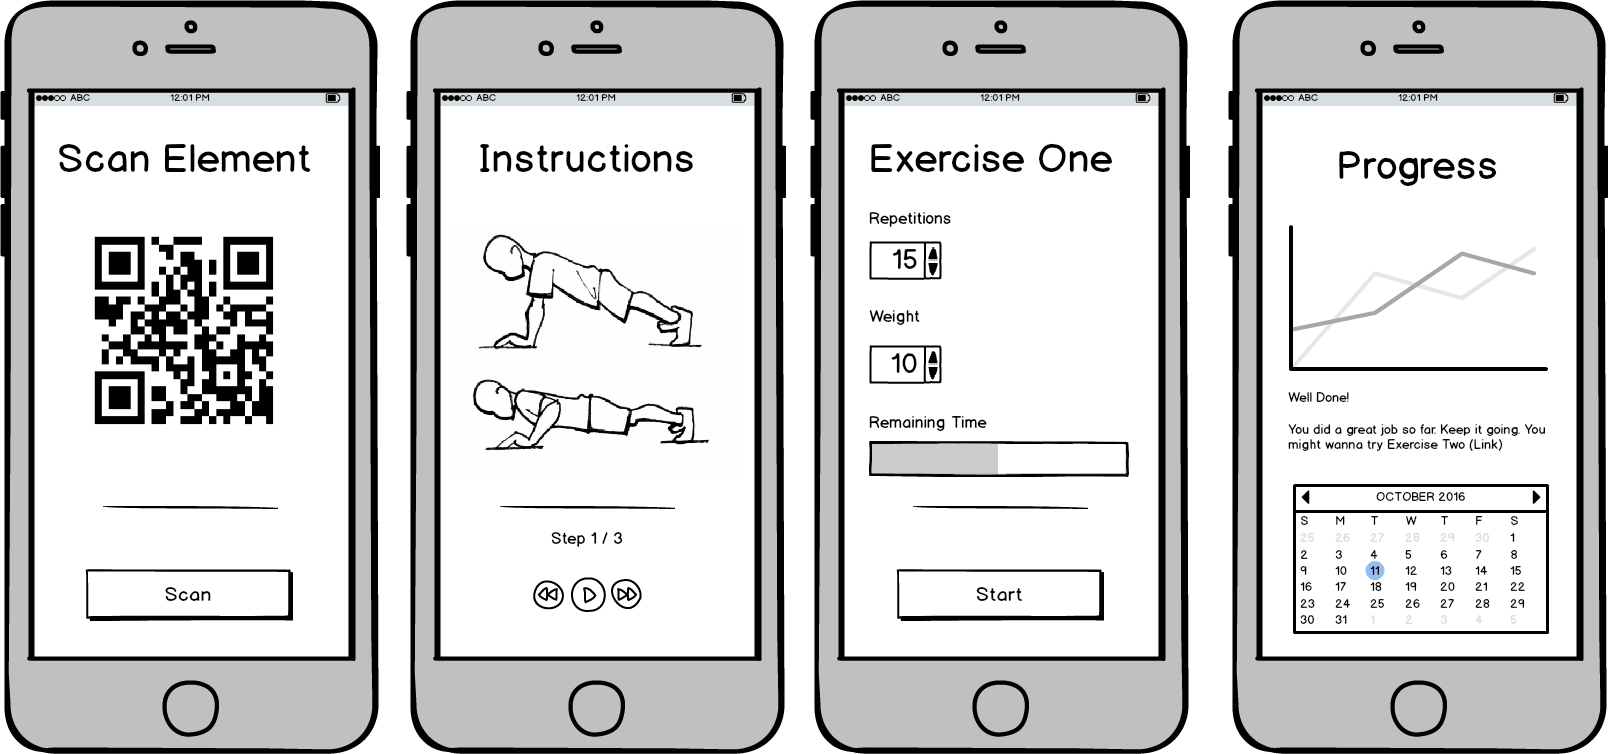
\includegraphics[width=0.5\linewidth]{images/app}
\caption{Wireframe der App}
\label{fig:app}
\end{figure}


\section{Markt und Kunden: das Zielgebiet}

\section{Konkurrenz: die Mitbewerber}

\section{Marketing: der Weg zum Markt}

\section{Beschaffung und Produktion: die Leistungserstellung}

\section{Management und Organisation: die Köpfe dahinter}

\section{Chancen und Risiken: eine ehrliche Bilanz}

\section{Finanzieller Teil: die nackten Zahlen}
% TODO ZKB KMU Check verwenden
% Das Finanzplanungstool der ZKB muss verwendet werden!
% Investitionsplan für 3 Jahre
% Eröffnungsbilanz + Planbilanzen (3 Jahre) + Planerfolgsrechnungen (3 Jahre) (nur normal case)
% Liquiditätsplan nur für erstes Jahr (pro Monat ausgewiesen)
% Mengengerüst, das den Berechnungen zugrunde liegt.

% TODO Was ist der Kunde bereit zu zahlen?

\section{Umsetzungsplan: die Realisierung}
Musste nicht bearbeitet werden

\clearpage
\appendix

% List of figures
\listoffigures

% List of tables
\listoftables

% Bibliography
\bibliographystyle{plain} 
\bibliography{literatur}

\end{document}